\documentclass[10pt]{article}
\usepackage{float}
\usepackage{listings}
\usepackage[french]{babel}
\usepackage[utf8x]{inputenc}
\usepackage{subcaption}
\usepackage{listings}
\usepackage{wrapfig}
\usepackage{color}
\usepackage{amsmath}
\usepackage{dsfont}
\usepackage{amsfonts}
\usepackage{hyperref}
\usepackage{mathtools}
\usepackage{graphicx}
\usepackage{caption}
\definecolor{dkgreen}{rgb}{0,0.6,0}
\definecolor{gray}{rgb}{0.5,0.5,0.5}
\definecolor{mauve}{rgb}{0.58,0,0.82}
\usepackage[table]{xcolor}
\usepackage{adjustbox}
\usepackage{multirow}
%opening
\definecolor{Gray}{gray}{0.85}




\lstset
{frame=tb,
	language=R,
	aboveskip=3mm,
	belowskip=3mm,
	showstringspaces=false,
	framexleftmargin=5mm,
	columns= fixed,
	numbers = left,
	basicstyle={\small\ttfamily},	
	numberstyle=\tiny\color{gray},
	keywordstyle=\color{blue},
	commentstyle=\color{dkgreen},
	stringstyle=\color{mauve},
	breaklines=true,
	breakatwhitespace=true,
	tabsize=3
}


\title{
	\normalfont \normalsize 
	\textsc{Université de Technologie de Compiègne\\ 
		SY09:Analyse des données et Data-Mining , P17} \\
	[10pt] 
	\rule{\linewidth}{0.5pt} \\[6pt] 
	\huge Rendu TP3\\
	\rule{\linewidth}{2pt}  \\[10pt]
}
\author{Zineb Slam, Oumaima Talouka}
\date{\normalsize \today}

\begin{document}
	{\let\newpage\relax\maketitle}	
	
		\begin{abstract}
			Dans ce rapport de TP3 nous allons étudier 2 méthodes d'apprentissage supervise: le Classifieur Euclidien et les K Plus Proches Voisins. Dans la première partie nous allons implémenter ces 2 méthodes en R. Ensuite nous allons évaluer leur performance avec différents jeux de données. Pour finir, nous allons calculer la règle de Bayes. Les fonctions ayant permis l'obtention de nos résultats sont jointes au rapport du TP.
		\end{abstract}
	
	\section{Classifieur euclidien, K plus proches voisins}
		\subsection{ Programmation}
		Nous avons essaye dans notre implémentation d'éviter les boucles au maximum possible, car celle ci réduisent les performances.
	La fonction \textit{ceuc.app } retourne les centres d'inertie de chaque classe pour l'ensemble d'apprentissage. La fonction \textit{rowsum} sur R nous a été très utile pour sommer les lignes de chaque classe .\\
	La fonction \textit{ceuc.val}  prédit la classe de chaque individu des données tests. Nous utilisons ici la fonction \textit{distXY} pour calculer la distance qui sépare chaque individu de chaque centres d'inertie.
	
	
		\subsubsection{ Test de fonctions}
		Pour tester nos fonctions nous allons représenter graphiquement les frontières de décision de chaque méthode en appelant les fonctions \textbf{\textit{front.ceuc}} et \textbf{\textit{front.val}} sur les données Synth1-40. On obtient les graphes représentés dans les figures ci-dessous.
			\begin{minipage}{.5\textwidth}
			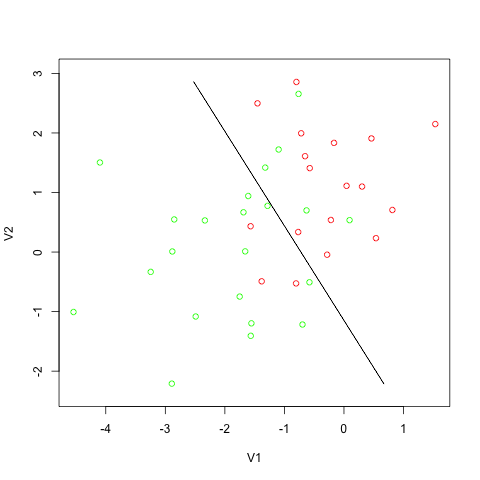
\includegraphics[width=45mm]{Figures/Exo1/front_ceuc.png}
			\captionof{figure}{Frontière de decision obtenue avec le Classifieur Eucledien}
			\label{fig:front_ceuc}
		\end{minipage}%
		\hspace{0.02\linewidth}
		\begin{minipage}{.5\textwidth}
		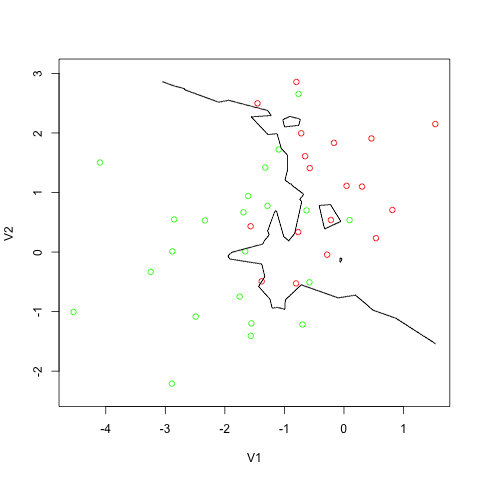
\includegraphics[width=45mm]{Figures/Exo1/front_kppv.png}
			\captionof{figure}{Frontière de décision obtenue avec la methode des K plus proches voisins (K=3) }
			\label{fig:front_kppv}
		\end{minipage}
		\vspace{0.2mm}
		
		Remarquons que la frontière de décision du classifieur Euclidien est linéaire tandis que celle du KPP est non linéaire.
		
			\subsection{ Évaluation des Performances} \label{section}
			
			\subsubsection{Estimation des paramètres}
			Dans cette partie on estime les moyennes $\mu_{k}$, les matrices de covariances $\Sigma_{k}$ ainsi que les proportions $\pi_{k}$ pour chaque jeu de données et pour chaque classe k. Nous utilisons pour cela 2 fonctions sur R: \textit{group\_by} et \textit{summarize}. La fonction \textit{group\_by} va grouper les données selon les classes z ensuite \textit{summarize} va calculer les paramètres pour chaque groupement. Dans cet exemple on obtient les paramètres de la variable V1.
			\begin{center}		
			\begin{tabular}{ | c | c | c | c | c |}
				\rowcolor{lightgray}
			& &  \multicolumn{3}{c|}{Estimation des Paramètres} \\
			\hline
			 Synth1 & k & $\mu_{k}$ & $\sum_{k}$ & $\pi_{k} $\\
			\hline
			\multirow{2}{*}{40}       &   1&     $\begin{pmatrix} -0.32\\1.09 \end{pmatrix}$                 &     $\begin{bmatrix} 0.68 & 0.12 \\ 0.12 & 1.01 \end{bmatrix}$      & 	0.45				\\\cline{2-5}
			
			      									        &   2&      $\begin{pmatrix} -1.883\\0.105 \end{pmatrix}$          &         $\begin{bmatrix} 1.37 & 0.32 \\ 0.32 &1.44 \end{bmatrix}$        & 			0.55  		\\  
			      									         
			\hline
			\hline
			\multirow{2}{*}{100}      &   1&    $\begin{pmatrix} 0.02\\0.82 \end{pmatrix}$              &           $\begin{bmatrix} 0.88 & -0.13 \\ -0.13 & 1.12 \end{bmatrix}$      & 		0.54	   \\\cline{2-5}
			      											
			      											 &   2&        $\begin{pmatrix} -1.96\\-0.13 \end{pmatrix}$          &         $\begin{bmatrix} 0.76 & -0.04 \\ -0.04 & 0.76 \end{bmatrix}$               & 			0.46		\\
		\hline
		\end{tabular} 
	\end{center}
		\begin{center}		
		\begin{tabular}{ | c | c | c | c | c |}
			\rowcolor{lightgray}
			& &  \multicolumn{3}{c|}{Estimation des Paramètres} \\
			\hline  
			 Synth1 & k & $\mu_{k}$ & $\sum_{k}$ & $\pi_{k} $\\
			\hline   											
			\multirow{2}{*}{500}        &   1&       $\begin{pmatrix} 0.13\\0.88 \end{pmatrix}$            &         	$\begin{bmatrix} 1.05 & 0.052 \\ 0.052 & 0.98 \end{bmatrix}$             & 			0.53		\\\cline{2-5}
			        											&   2&         $\begin{pmatrix} -1.88\\-0.08 \end{pmatrix}$         &  
			        											$\begin{bmatrix} 0.97 & -0.11 \\ -0.11 & 0.98 \end{bmatrix}$                      & 		0.47		\\
		
			\hline
			\hline
			\multirow{2}{*}{1000}         &   1&   $\begin{pmatrix} -0.01\\0.91 \end{pmatrix}$           &        	$\begin{bmatrix} 0.97 & 0.06  \\ 1.08 & 0.06 \end{bmatrix}$          & 		0.50		\\\cline{2-5}
			         										&   2&       $\begin{pmatrix} -1.96\\0.02 \end{pmatrix}$            &    $\begin{bmatrix} 0.99 & 0.02 \\0.02 & 0.94 \end{bmatrix}$                  & 	0.50				\\
			\hline
			\end{tabular}
		\end{center}
	
			\subsubsection{Calcul du taux d'erreur du classifieur Euclidien }
			Dans cette partie nous allons tester les performances de chacun des algorithmes programmes precedement en utilisant le critère de l'erreur qu'on exprime comme:
			\begin{center}
			$Erreur = \frac{1}{N} \sum_{i=1}^{n} {\mathds{1} \hat{z}_{i}  \neq z_{i}}$
			\end{center}
		Avec $z_{i}$ la vrai valeur de z et $\hat{z}_{i}$ la valeur calculée a partir de l'algorithme. N est le nombre d'individus. $\mathds{1} \hat{z}_{i}  \neq z_{i}$ = 1 si $\hat{z}_{i}  = z_{i}$, 0 sinon.
		Après avoir calculé l'erreur qu'on suppose suit une loi normale de moyenne $\mu_{\epsilon}$ et de variance $\sigma_{\epsilon}$, on peut calculer l'intervalle de confiance exprimé ci-dessous.
		\begin{center}
		$Ic = [\mu_\epsilon - t \frac{\sigma_{\epsilon}^2}{\sqrt{N}}, \mu_\epsilon + t \frac{\sigma_{\epsilon}^2}{\sqrt{N}}]$
		\end{center}
	
		On choisit un niveau de confiance t de 95\%. Notons ici que  $\mu$ et $\sigma$ sont ceux calculés pour les différentes valeurs de $\epsilon$ et non ceux du jeu de données. Autre point a remarquer est le N qui est ici le nombre d'individus , or comme on a séparé nos jeux de données en un ensemble d'application et un ensemble de test, on veillera a mettre le nombre d'individus correspondant en fonction si c'est l'intervalle de confiance  d'application ou test. D'après l'énoncé en utilisant la fonction \textit{separ1} napp =$\frac{2n}{3}$  et ntst=$\frac{n}{3}$ n étant le nombre total d'individus du jeu de donnée.
			
			On fait tourner 20 fois le classifier Euclidien ainsi que le KPP puis on calcules les erreurs obtenus. Les résultats obtenus pour les jeux de données sont affichés dans Le tableau qui suit.
			\begin{center}		
				\begin{tabular}{ | c | c| c | c | c |}
						\rowcolor{lightgray} 
				   	&  \multicolumn{4}{|c|}{ Performance du  Classifieur Euclidien}\\
					
					\hline
					 Synth1  &  $\epsilon_{app}$ &  $Ic_{app}$&  $\epsilon_{test}$ &  $Ic_{test}$  \\
					\hline
					\multirow{1}{*}{40}   & 0.23  & $[0.218, 0.234]$& 0.18      & 	$[0.155, 0.205]$ \\
															
					\hline
					\multirow{1}{*}{100}      &0.085  &   $[0.083, 0.088  ]$& 0.102     & 	$[0.093, 0.111]$  \\
				
					\hline
					\multirow{1}{*}{500}     & 0.132 &   $[0.131, 0.132]$& 0.134    & 	$[0.132, 0.136]$	\\
				
					\hline
					\multirow{1}{*}{1000}    & 0.140     & $[0.140, 0.141]$ &  0.147   & $[0.146, 0.147]$  	\\
				
					\hline
				\end{tabular}
			\end{center}
		\vspace{1.5mm}
			En remarquant les intervalles de confiance on remarque que l'erreur d'apprentissage est inférieure a celle du test ce qui est normal vu qu'on entrainé le modèle avec ses données. On remarque aussi que plus le nombre d'individus augmente  plus l'intervalle de confiance diminue diminue ce qui est logique car avec plus de données dans le modèle d'apprentissage apprend mieux les données et donc pourra mieux classer l'ensemble de test. Notons ici le faible taux d'erreur qu'on a obtenu avec les donnees \textbf{Synth1-100}, ce qui peut revenir a la génération de données.
			 
				\subsubsection{Le nombre Optimal de voisins du KPP }
				Le nombre optimal de voisins qu'en peut obtenir en ayant l'ensemble d'apprentissage comme ensemble de validation (Xval = Xapp) est toujours de 1 puisque le plus proche voisin d'un individu est lui même et donc chaque individu sera attribue a sa vraie classe (zval = zapp). L'erreur sera donc nulle dans ce cas et le modèle sera alors biaisé, d'ou l'intérêt d'avoir un ensemble d'apprentissage, un ensemble de validation pour déterminer le meilleur k puis un ensemble de test.
			
				\subsubsection{Calcul du taux d'erreur du KPP }
				De la même manière qu'avec le Classifieur Euclidien on obtient les résultats des taux d'erreurs ci-dessous. Notons ici que la notion d'erreur d'apprentissage n'a pas de sens ici car le modèle n'a pas besoin d'apprendre d'abord sur des données puis tester, il fait tout en un seul appel de fonction.
		\begin{center}		
			\begin{tabular}{ | c | c | c |}
				\rowcolor{lightgray} 
				  &  \multicolumn{2}{c}{Performance du KPP}\\
				
				\hline
				Jeu de données Synth1 &   $\epsilon_{test}$ &  $Ic_{test}$\\
				\hline
				\multirow{1}{*}{40}       &0.295  & $[0.253, 0.337]$ 			 \\
				
				\hline
				\multirow{1}{*}{100}      & 0.104 	& $[0.094, 0.114]$  \\
				
				\hline
				\multirow{1}{*}{500}      &  0.152  & 	$[0.149, 0.154]$	\\
				
				\hline
				\multirow{1}{*}{1000}      & 0.146  & 	$[0.144, 0.147]$ 		\\
				
				\hline
			\end{tabular}
		\end{center}
	

			\subsection{Analyse des résultats } 
			 En comparant les 2 méthodes on remarque que l'erreur ainsi que les intervalles de confiance du Classifier Euclidien sont bien inférieur a ceux de la méthode des KPP. On a donc peut être des... 
			
				\subsubsection{ Jeux de données Synth2-1000}
				
					\begin{center}		
					\begin{tabular}{ | c | c | c | c | c |}
						\rowcolor{lightgray} \multicolumn{5}{|c|}{Estimation des Paramètres} \\
						\hline
						Jeu de données & k & $\mu_{k}$ & $\sum_{k}$ & $\pi_{k} $\\
						\hline
						\multirow{2}{*}{Synth2-1000}       &   1&  $ \begin{pmatrix} 3.018\\-0.0063 \end{pmatrix} $             &     $\begin{bmatrix} 0.9904 & 0.1131 \\ 0.1131 & 1.092 \end{bmatrix}$      & 	0.52	     	\\\cline{2-5}
																	&   2&   $\begin{pmatrix} -2.142\\-0.0265 \end{pmatrix}$                 &     $\begin{bmatrix} 4.435 & -0.154 \\ -0.154 & 1.030 \end{bmatrix}$      & 	0.48				\\
						\hline
					
					\end{tabular}
				\end{center}
			
				Grâce a cette estimation on peut remarquer que \[ \lim \pi_{1} = \lim \pi_{1} = 0.5 \quad \mu_{1} = (3, 0)^{T} 
			\quad \mu_{2} = (-2, 0)^{T} \quad \Sigma_{1} = \begin{bmatrix} 1 & 0 \\ 0 & 1\end{bmatrix} \quad \Sigma_{1} = \begin{bmatrix} 5 & 0 \\ 0& 1\end{bmatrix}\]
				\begin{center}		
				\begin{tabular}{ | c | c | c || c | c |}
						\rowcolor{lightgray} 
			 	 &  \multicolumn{4}{c||}{ Performance du Classifier Euclidien}  \\
					\hline
					Jeu de données &   $\epsilon_{app}$ & $Ic_{app}$ & $\epsilon_{test}$ & $Ic_{test}$\\
					\hline
					\multirow{1}{*}{Synth2-1000}     &         0.061   & $[0.061, 0.062]$		&0.063   &		$[0.062, 0.064]$	 \\
					
					\hline
					
				\end{tabular}
			\end{center}
	
		
		\begin{center}		
			\begin{tabular}{ | c | c | c |}
				\rowcolor{lightgray} 
				&  \multicolumn{2}{|c|}{Performance du KPP}\\
				
				\hline
				Jeu de données &   $\epsilon_{test}$ &  $Ic_{test}$\\
				\hline
				\multirow{1}{*}{Synth2-1000}       &0.062   & $[ 0.061, 0.063]$ 			 \\
				\hline
			\end{tabular}
		\end{center}
				Contrairement aux jeux de données \textit{Synth1-n} on remarque le KPP semble donner des résultats légèrement meilleures avec \textit{Synth2}.
				\subsubsection{ Jeux de données réelles: Pima \& Breast Cancer}
				
			
				
				
				\begin{center}		
				\begin{tabular}{ | c | c | c || c | c |}
					\rowcolor{lightgray} 
					&  \multicolumn{4}{c||}{ Performance du Classifier Euclidien}  \\
					\hline
					Jeu de données &   $\epsilon_{app}$ & $Ic_{app}$ & $\epsilon_{test}$ & $Ic_{test}$\\
					\hline
					\multirow{1}{*}{Pima}     &     0.252   & $[0.251, 0.252]$		&0.236     &		$[0.234, 0.238 ]$	 \\
					\hline
					\multirow{1}{*}{Cancer}     &    0.040   & $[0.040, 0.0407]$& 0.039    &		$[0.038, 0.039]$	 \\
					\hline
					
				\end{tabular}
			\end{center}
				
				
					\begin{center}		
					\begin{tabular}{ | c | c | c |}
						\rowcolor{lightgray} 
						&  \multicolumn{2}{|c|}{Performance du KPP}\\
						
						\hline
						Jeu de données &   $\epsilon_{test}$ &  $Ic_{test}$\\
						\hline
						\multirow{1}{*}{Pima}       & 0.248 & $[0.245, 0.250]$ 			 \\
						\hline
							\multirow{1}{*}{Cancer}       &0.040    & $[0.039, 0.042]$ 			 \\
						\hline
					\end{tabular}
				\end{center}
				
				
				
	
	\section{Règle de Bayes}
	\subsection{Loi Marginale}
	La première remarque qu'on peur faire concernant les paramètres des données de Synth1n et Synth2 est que les matrices de variances $\sum_{1}$ et $\sum_{2} $ sont diagonales, donc les covariances COV(V1, V2) =0. Ainsi on peut en déduire que les variables sont indépendantes. Cette remarque va nous être utile dans le calcul de la loi marginale de chaque classe $\omega_{1} $ et $ \omega_{2}$. Ainsi on peut écrire:
	\begin{equation}
	\begin{split}
		f(X^{1}, X^{2}| \omega_{1}) = f(X^{1}|\omega_{1})  f(X^{2}|\omega_{1})\\
		f(X^{1}, X^{2}| \omega_{2}) = f(X^{1}|\omega_{2})  f(X^{2}|\omega_{2})
		\end{split}
		\label{1}
	\end{equation}
	
Les individus de la classe 1 et 2 suivent une loi normale bivariee, donc on peut écrire: 
	\begin{equation}
f(X|\omega_{k}) = \frac{1}{\sqrt{2\pi|\Sigma_{k}|}} exp(-\frac{1}{2} (x-\mu_{k})^{T} \Sigma_{k}^{-1} (x-\mu_{k})) \quad avec \quad   x = \begin{pmatrix} x_{1} \\ x_{2} \end{pmatrix} 
	\label{2}
	\end{equation}

\subsubsection{Synth1}
Dans le cas des jeux de données Synth1 nous avons \[\mu{1}= \begin{pmatrix} 0 \\ 1 \end{pmatrix} \quad \mu_{2}= \begin{pmatrix} -2 \\ 0 \end{pmatrix}, \quad  \Sigma = \Sigma_{1} = \Sigma_{2} = \begin{pmatrix} 1 & 0 \\ 0 & 1	\end{pmatrix} \quad et  \quad \pi_{1} = \pi_{2} = 0.5\]


D'après la formule  \refeq{2} on peut alors exprimer les densités comme suit:\\
\begin{equation}
\begin{tabular}{c | c}
	$f_{X^{1}}(x_{1}|\omega_{1}|) = \frac{1}{\sqrt{2\pi}}exp(-\frac{1}{2} x_{1}^{2})$ & 	$f_{X^{1}}(x_{1}|\omega_{2}|) = \frac{1}{\sqrt{2\pi}}exp(-\frac{1}{2} (x_{1}+2)^{2})$\\\\
	$f_{X^{2}}(x_{2}|\omega_{1}|) = \frac{1}{\sqrt{2\pi}}exp(-\frac{1}{2} (x_{2}-1)^{2})$ & 	$f_{X^{2}}(x_{2}|\omega_{2}|) = \frac{1}{\sqrt{2\pi}}exp(-\frac{1}{2} x_{2}^{2})$\\
\end{tabular}
\label{3}
\end{equation}

On obtient ainsi selon \eqref{1} les densités jointes de chacune des classes ci-dessous:
\begin{equation}
\begin{split}
		f_{X^{1}, X^{2}}(x|\omega_{1}) = \frac{1}{2\pi} exp(-\frac{1}{2}(x_{1}^2 + (x_{2}-1)^{2} ))  \\
f_{X^{1}, X^{2}}(x|\omega_{2}) = \frac{1}{2\pi} exp(-\frac{1}{2}(x_{2}^2 + (x_{1}+2)^{2} ))
\end{split}
\label{4}
\end{equation}


\subsubsection{Synth2}
Dans le cas des jeux de donnes Synth2 nous avons:
\[\mu{1}= \begin{pmatrix} 3 \\ 0 \end{pmatrix} \quad \mu_{2}= \begin{pmatrix} -2 \\ 0 \end{pmatrix}, \quad   \Sigma_{1} = \begin{pmatrix} 1 & 0 \\ 0 & 1	\end{pmatrix}  \quad  \Sigma_{2} = \begin{pmatrix} 5 & 0 \\ 0 & 1	\end{pmatrix}  et  \quad \pi_{1} = \pi_{2} = 0.5\]

Les densités des variable pour chaque classe sont alors:
\begin{equation}
\begin{tabular}{c | c}
$f_{X^{1}}(x_{1}|\omega_{1}|) = \frac{1}{\sqrt{2\pi}}exp(-\frac{1}{2} (x_{1} -3 )^{2})$ & 	$f_{X^{1}}(x_{1}|\omega_{2}|) = \frac{1}{\sqrt{10\pi}}exp(-\frac{1}{10} (x_{1}+2)^{2})$\\\\
$f_{X^{2}}(x_{2}|\omega_{1}|) = \frac{1}{\sqrt{2\pi}}exp(-\frac{1}{2} x_{2}^{2})$ & 	$f_{X^{2}}(x_{2}|\omega_{2}|) = \frac{1}{\sqrt{10\pi}}exp(-\frac{1}{2} x_{2}^{2})$\\
\end{tabular}
\label{5}
\end{equation}

On obtient ainsi selon \eqref{1} les densités jointes de chacune des classes ci-dessous:
\begin{equation}
\begin{split}
f_{X^{1}, X^{2}}(x|\omega_{1}) = \frac{1}{2\pi} exp(-\frac{1}{2}(x_{1}-3)^2 - \frac{1}{2}x_{2}^2       )  \\
f_{X^{1}, X^{2}}(x|\omega_{2}) = \frac{1}{10\pi} exp(-\frac{1}{10}(x_{1}+2)^{2}  - \frac{1}{2}x_{2}^{2})
\end{split}
\label{6}
\end{equation}


\subsection{Courbe d'iso-densité}
Une courbes d'iso-densité correspond a la régions ou la densité est constante.

\subsubsection{iso-densité de Synth1}
\textbf{Pour la classe $\omega_{1}$} $f(X^{1}, X^{2}|\omega_{1}) = C_{1} \quad avec \quad C_{1} constante$
\begin{equation}
\begin{split}
exp(-\frac{1}{2} (x_{1}-\mu_{1})^{2} - \frac{1}{2}(x_{2} - \mu{1})^{2})  = 2 \pi \sigma_{11}^{2} \sigma_{22}^{2} C_{1}
\\
(x_{1} - \mu_{1})^{2} + (x_{2} - \mu_{1})^{2} = -2ln(2 \pi \sigma_{11}^{2} \sigma_{22}^{2} C_{1})
\\
x_{1}^{2} + (x_{2} - 1)^{2} = -2 ln(2\pi C_{1})
\end{split}
\label{7}
\end{equation}

 L'équation \eqref{5} obtenue est une équation de cercle de centre $\mu_{1} = \begin{pmatrix} 0 \\ 1\end{pmatrix} $ et de rayon $R^{2} = -2 ln(2\pi C_{1})$.\\
 
 \textbf{De même pour la classe $\omega_{2}$} $f(X^{1}, X^{2}|\omega_{2}) = C_{2} \quad avec \quad C_{2} constante$
 \begin{equation}
 \begin{split}
 (x_{1} - \mu_{2})^{2} + (x_{2} - \mu_{2})^{2} = -2ln(2 \pi \sigma_{11}^{2} \sigma_{22}^{2}C_{2}) 
 \\
 (x_{1} + 2)^{2} + x_{2}^{2} = -2ln(2\pi C_{2})
 \label{8}
\end{split}
 \end{equation}
 
 On obtient encore une fois l'équation de cercle de centre $\mu_{2} = \begin{pmatrix} -2 \\ 0\end{pmatrix} $ et de rayon $R^{2} = -2 ln(2\pi C_{2})$.\\


\subsubsection{iso-densité de Synth2}
\textbf{Pour la classe $\omega_{1}$} $f(X^{1}, X^{2}|\omega_{1}) = C_{3} \quad avec \quad C_{3} constante$
\begin{equation}
\begin{split}
exp(-\frac{1}{2} (x_{1}-\mu_{1})^{2} - \frac{1}{2}x_{2}^{2})  = 2 \pi \sigma_{11}^{2} \sigma_{22}^{2} C_{3}
\\
(x_{1} - \mu_{1})^{2} +  x_{2}^{2} = -2ln(2 \pi \sigma_{11}^{2} \sigma_{22}^{2} C_{3})
\\
(x_{1} - 3)^{2} + x_{2}^{2} = -2 ln(2\pi C_{3})
\end{split}
\label{9}
\end{equation}

L'équation obtenue est une équation de cercle de centre $\mu_{1} = \begin{pmatrix} 3 \\ 1\end{pmatrix} $ et de rayon $R^{2} = -2 ln(2\pi C_{2})$.\\

\textbf{De même pour la classe $\omega_{2}$} $f(X^{1}, X^{2}|\omega_{2}) = C_{4} \quad avec \quad C_{4} constante$
\begin{equation}
\begin{split}
exp(-\frac{1}{10} (x_{1}-\mu_{1})^{2} - \frac{1}{2}(x_{2}-\mu_{2})^{2})  = 10 \pi \sigma_{11}^{2} \sigma_{22}^{2} C_{4}
\\
(x_{1} - \mu_{1})^{2} +  5(x_{2}-\mu_{2})^{2}  = -10ln(10 \pi \sigma_{11}^{2} \sigma_{22}^{2} C_{3})
\\
(x_{1} - 3)^{2} + 5x_{2}^{2} = -10 ln(50\pi C_{3})
\\
(x_{1} + 2)^{2} + x_{2}^{2} = -10ln(50\pi C_{2})
\label{10}
\end{split}
\end{equation}

On obtient encore une fois l'équation de cercle de centre $\mu_{2} = \begin{pmatrix} -2 \\ 0\end{pmatrix} $ et de rayon $R^{2} = -2 ln(2\pi C_{2})$.\\


\subsection{Règle de Bayes}
La règle de Bayes s'exprime de la manière:

\[\delta^{*}(x) = \begin{cases} \omega_{1} & si  \quad \Pr(\omega_{1}|x)>  \Pr(\omega_{2}|x) \\
	\omega_{2} & sinon \end{cases}\]
\begin{equation}
\begin{split}
 \iff \delta^{*}(x) = \omega_{1} \quad & si \quad  \frac{f_{X}(x|\omega_{1})}{f_{X}(x)} \pi_{1}> \frac{f_{X}(x|\omega_{2})}{f_{X}(x)}\pi_{2} \\ 
\iff \delta^{*}(x) = \omega_{1} \quad & si \quad  \frac{f_{X}(x|\omega_{1})}{f_{X}|\omega_{2}(x)} > \frac{\pi_{2}}{\pi_{1}} \\ 
\end{split}
\label{9}
\end{equation}
 Dans la suite nous notons $f_1(x) = f_{X}(x|\omega_{1})$ et $f_2(x) = f_{X}(x|\omega_{2})$

\subsubsection{Synth1}
D'après les densités calculées dans \eqref{4} on obtient: \[\frac{f_{1}(x)}{f_{2}(x)} = exp(2x_{1} + x_{2} + \frac{3}{2})\]
On peut donc exprimer l'inéquation \ref{7} de facon linaire en introduisant le \textit{log} , ainsi on a
\begin{equation}
\begin{split}
2x_{1} + x_{2} > ln\frac{\pi_{2}}{\pi_{1}} - \frac{3}{2}   \quad \frac{\pi_{2}}{\pi_{1}} = 1 \\
x_{2} >  -2x_{1} - \frac{3}{2}
\label{10}
\end{split}
\end{equation}

Ainsi La règle de Bayes attribuera l'individu a la classe 1 si \eqref{10} est vérifiée si non a la classe 2. Nous obtenons donc une frontière linéaire si les 2 matrices de covariances sont égales. Nous avons représenté cela de manière graphique sur les données Synth1 avec n=40 et n=50 en utilisant ggplot.\\

			\begin{minipage}{.5\textwidth}
	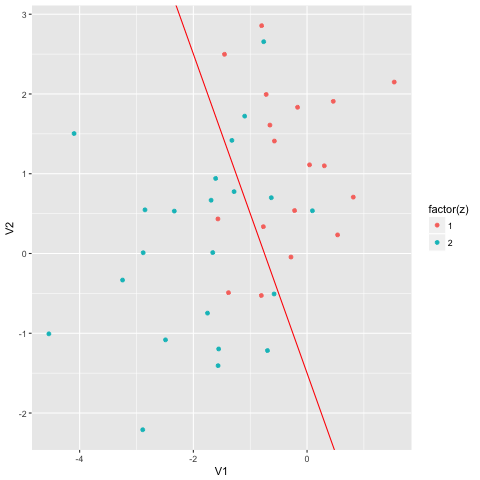
\includegraphics[width=45mm]{Figures/Exo2/linear_synth140.png}
	\captionof{figure}{Frontière de decision Lineaire pour Synth140}
	\label{fig:front_ceuc}
\end{minipage}%
\hspace{0.02\linewidth}
\begin{minipage}{.5\textwidth}
	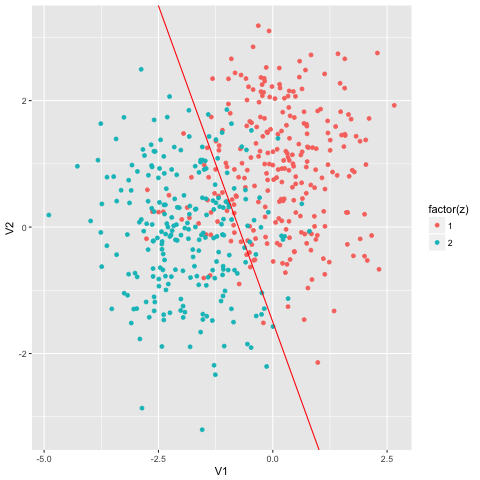
\includegraphics[width=45mm]{Figures/Exo2/linear_synth1500.png}
	\captionof{figure}{Frontière de decision Lineaire pour Synth1500}
	\label{fig:front_kppv}
\end{minipage}

\subsubsection{Synth2}
D'après les densités calculées dans \eqref{4} on obtient: \[\frac{f_{1}(x)}{f_{2}(x)} = 5exp(-\frac{4}{10}x_{1}^{2} + \frac{34}{10} x_{1} - \frac{41}{10})\]

On obtient ainsi l'inéquation: \[-4x_{1}^{2}  - 34x_{1} - 41 > -10ln5\]
En résolvant cette inéquation de second degrés par $\Delta = b^{2} - 4ac$ on obtient 2 solutions
\[k_{1} = 0,342 \quad k_{2} = -8.842 \]

Ainsi lorsqu'on a des matrices de covariances différentes on obtient une frontière de décision quadratique. Cette frontière est représentée  ci-dessous de 2 manières différentes pour les jeux de données Synth2 en utilisant \textbf{ggplot\textit{}} sur R et stat\_function pour dessiner la fonction quadratique.\\

\begin{minipage}{.5\textwidth}
	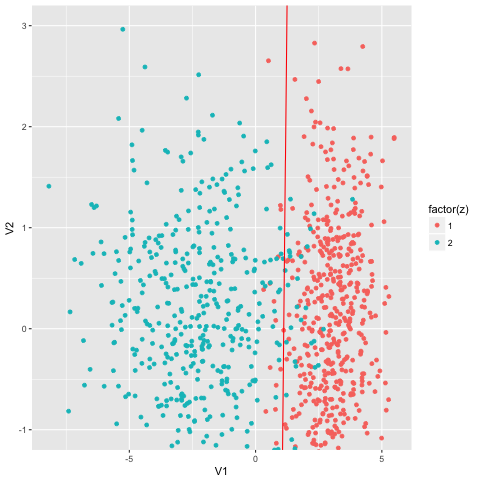
\includegraphics[width=45mm]{Figures/Exo2/curve_synth2.png}
	\captionof{figure}{Frontière de decision Quadratique pour Synth2}
	\label{fig:front1_synth2}
\end{minipage}%
\hspace{0.02\linewidth}
\begin{minipage}{.5\textwidth}
	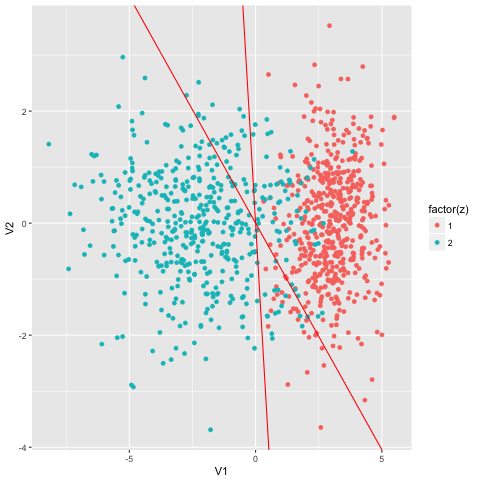
\includegraphics[width=45mm]{Figures/Exo2/linear2_synth2.png}
	\captionof{figure}{Frontière de decision  pour Synth2}
	\label{fig:front2_synth2}
\end{minipage}
\vspace{0.2mm}
La figure \ref{fig:front1_synth2} montre la frontière de décision entre les 2 classes. Cette frontière qui est en effet une courbe apparait ici comme linéaire car on a restreint l'échelle a celle de nos données.

\subsection{Erreur de Bayes}
L'erreur de Bayes  est la plus petite erreur possible que peut atteindre une règle $\delta$ utilisant uniquement X. 
\subsubsection{Synth1}
Dans le cas des jeux de données de \textit{Synth1n} les matrices de covariances sont égales $(\sigma_{k} = \sigma)$ et les probabilités a priori de chaque classe aussi  ($\pi_{1} = \pi{2}$). Avec ces conditions, l'erreur de Bayes s'écrit de la forme: \[ \epsilon^{*} = \phi(-\frac{\Delta}{2}) . \]
ou $\phi$ est la fonction de répartition de la loi normale (univariee) centrée réduite  et $ \Delta^{2}   = (\mu_{2} - \mu_{1})^{T} \sigma^{-1} (\mu_{2}  - \mu_{1})$ est la \textit{distance au carrée de Mahalanobis}.\\
On obtient alors $\Delta^{2} = 5$, d'ou $\Delta = \sqrt{5} $ Ainsi: 

\begin{align}
 \epsilon^{*}  &=  \phi(-\frac{\sqrt{5}}{2}) \cr
& =  Pr(x \leq -\frac{\sqrt{5}}{2}) \cr
 &= 1 - \Pr(x \leq \frac{\sqrt{5}}{2})\cr
 & = 1 - 0.86\cr
 \epsilon^{*}  & = 0.13
\end{align}
On remarque ainsi que cette erreur est relativement proche a l'erreur de test $\epsilon_{test}$ du classifieur Euclidien calculée dans la section \ref{section}



\subsubsection{Synth2}
Dans le cas general ou les matrices de covariances ne sont pas égales on peut déduire une borne supérieure de l'erreur de Bayes. Dans la page 98 du  poly on trouve l'expression de cette borne dans le  cas de 2 classes:
\[ \epsilon^{*} \leq \sqrt{\pi_{1}\pi_{2}}  \exp{-\Delta_{B}^{2}} \]
Avec $\Delta_{B}^{2}$ la distance de Bhattacharyya entre les 2 classes et qui s'exprime comme 
\[  \Delta_{B}^{2} = \frac{1}{8} (\mu_{2} - \mu_{1})^{T}  (\frac{\Sigma_{1} + \Sigma_{2}}{2})^{-1} (\mu_{2} - \mu_{1}) + 
\frac{1}{2} ln\frac{|\frac{\Sigma_{1}+\Sigma_{2}}{2}|}{\sqrt{|\Sigma_{1}| |\Sigma_{2}|}} \]

On obtient alors $\Delta_{B}^{2} = \frac{25}{24} +\frac{1}{2} ln(\frac{3}{5} ) = 0.79$
\[  \epsilon^{*} \leq 0.45\]

Ainsi l'erreur maximale que peut atteindre l'erreur de Bayes est 0.45

\section{Conclusion}
	\end{document}